%%%%%%%%%%%%%%%%%%%%%%%%%%%%%%%%%%%%%%%%%%%%%%%%%%%%%%%%%%%%%%%%
%
%  Template for creating scribe notes for MLPM2013.
%
%  Fill in your name, lecture number, lecture date and body
%  of scribe notes as indicated below.
%
%%%%%%%%%%%%%%%%%%%%%%%%%%%%%%%%%%%%%%%%%%%%%%%%%%%%%%%%%%%%%%%%


\documentclass[11pt]{article}


\pagestyle{plain}
\usepackage{tikz}
\usepackage{amssymb}
\usetikzlibrary{calc}
\usetikzlibrary{positioning}
\usepackage{algorithm}
\usepackage[noend]{algpseudocode}
\usepackage{amsmath}
\begin{document}




\section*{Approach}
The present research aims towards optimizing player experience through intelligent game level generation. State of the art facial expression recognition software is used to track players' emotions  throughout a game session, while its output serves as input in a gradient ascent optimization system that on-line determines the game difficulty level. The main challenge faced following this approach is accurate interpretation of in-game users' expressions and further mapping of these into game difficulty levels. 

\subsection*{Emotion tracking}
Player emotions are observed through the entire duration of a game, but are taken into account independently for each chunk. Namely, user expressions detected in chunk $c$ only affect the difficulty level of that particular chunk. In that way, personalization is achieved at the core components of the game while a wide variety of difficulty levels can be reached within a single segment, adapting to the users' preferences regarding game chunks.

Furthermore, user emotions are taken into consideration during in-game death, which leads to a short game pause of a few seconds. It has been observed that during that period, users show high emotional activity, which we consider essential for the calibration of game difficulty.	It is a fact that a vast majority of the users tend to keep a neutral expression during game activity while most emotional "bursts" occur while players experience in-game death. As shown in Figure \ref{fig:emotions10seg}, neutral is the dominating emotion recorded in almost the entire course of 10 game segments, while spikes and bursts of anger, happiness and sadness are also present.

\begin{figure}
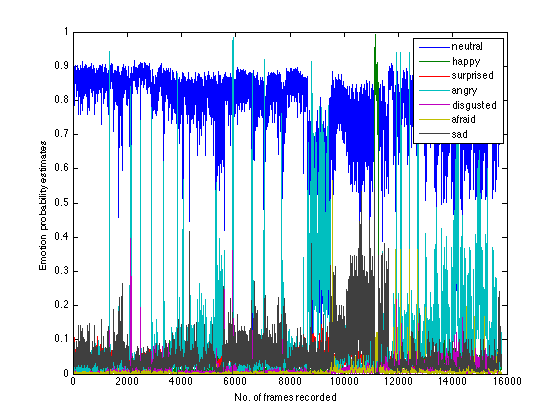
\includegraphics[scale=0.6]{emotions.png}
\caption{Player emotions over the course of 10 segments.}
\label{fig:emotions10seg}
\end{figure}


In practical terms, the InSight facial expression recognition software records approximately 15 frames per second, alongside each one of them a vector of decimal numbers representing a probability distribution over 7 different emotions: \{Neutral, Happiness, Disgust, Anger, Fear, Sadness, Surprise\}. Moreover, the duration of a chunk varies from 2 to 10 seconds, depending on difficulty level, resulting in a total of 30 to 150 vectors for each game chunk individually. These emotion vectors are averaged at the end of each chunk, giving an estimate of a user's emotional status.

Lastly, during the first segment of each game session, the variance of the entirety of emotions observed is calculated, from which a factor $\alpha = 1 - var(E)$ is derived. $\alpha$ is an important feature of the gradient ascent algorithm, and is aiming towards providing an "emotionality" measure for each user. In particular, the less emotional a user is, the higher an impact a burst of emotions should have on the calculations of the level generator.

\subsection*{Gradient Ascent Optimization}

In order to accurately map emotion vectors to in-game difficulty levels, we introduce a Gradient Ascent Optimization (GAO) implementation. The goal of GAO is to exploit the users' facial expressions in order to adapt the game to their preferences and achieve an optimal level of difficulty setup.

The way GAO is implemented is quite simple and straightforward; After each completion of a game segment, the emotion estimations are retrieved for each individual chunk. The emotions taken into consideration are Neutral, Happiness and Anger, which have been proven to be the most likely to be expressed by users during a game session. The emotion which shows the highest difference between the respective chunks of the currently finished and previously completed segment, is the one that defines the step taken in the current iteration of GAO. An increase in happiness should analogously increase the chunk's difficulty, while an increase in anger or neutrality should decrease it. In theory, after several segments are completed, a stability in the user's expressions should also result in a convergence to an optimal difficulty level setting. As observed in Figure \ref{fig:difficulties10seg}, starting from an "easy" difficulty setting for each game chunk, GAO adapts and converges according to the player's preferences in the course of 10 segments.

\begin{figure}
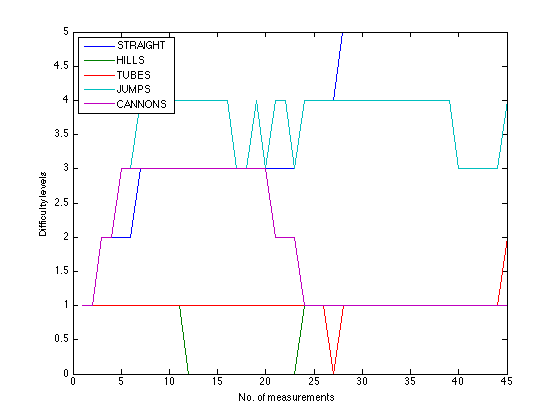
\includegraphics[scale=0.5]{difficulties.png}
\caption{Difficulty adaptations during 10 game segments.}
\label{fig:difficulties10seg}
\end{figure}


The algorithm is provided step by step below: 


\begin{algorithm}
\caption{Gradient Ascent Optimization for Personalized Mario}\label{euclid}
\begin{algorithmic}[1]
\Procedure{GAOptimize}{$e_t,e_{t-1}$}\Comment{Emotion vectors of current and previous segment}

   \State $\alpha\gets 1-Var(e_1)$\Comment{compute alpha (first segment)}
   \State $\delta \gets \alpha*5$\Comment{scale to difficulty space [-5...5]}
      \For{$each : Section$}

      \State $\epsilon\gets argmax|e_t-e_{t-1}|$ 
      \State $nextAction\gets\epsilon*\delta$
      \If{$\epsilon\in\{angry,neutral\}$}
      \State{$nextAction \gets -nextAction$}
      \EndIf
       \State{$nextDifficulty\gets previousDifficulty + nextAction$}
      \State \textbf{return} $newDifficulty$
   \EndFor
   
\EndProcedure
\end{algorithmic}
\end{algorithm}

\subsection*{Heuristics}
In order to boost the functionality of GAO, heuristic values are introduced in special occasions. 

Generally, as mentioned before, users tend to show highly neutral expressions during game activity, especially in low difficulty level settings. In order to prevent "stalling" of the game in the same difficulty setup because of lack of emotionality, we introduce a heuristic threshold $\tau = 0.8\alpha$ which derives from our observations on user behavior (see Figure \ref{fig:emotions10seg}). If, by the end of a segment, the level of neutrality of a user during a chunk is higher than $\tau$, the level generator will force an increase in difficulty by a unit (+1) measure in the next segment's respective chunk.

On the other hand, high difficulty levels could impose an unpleasant experience on users. In order to avoid game abandonment resulting from an inappropriately high difficulty setup, a heuristic value is applied onto emotions observed during in-game death. A threshold $\phi = 5\alpha\times\epsilon_{anger}$  is introduced regarding the anger measurement during death. The chunk in which death happened will instantly drop by $round(\phi)$ units of difficulty in order to reduce user anger and boost user progress in the game. Note that $\epsilon_{anger} \in \{0...1\}$ is multiplied by $5$ in order to directly map emotion probability scale into game difficulty scale.

\section{Result tables (4 segments)}
The tables below show the average preferences in difficulty and emotion estimates for 10 players, 3 different setups and 4 segment game sessions.

\begin{table}
\small
\begin{tabular}{l|{c}*6r}
Difficulty & Neutral & Happy & Surprised & Angry & Disgusted & Afraid & Sad\\ 
\hline \\
 Easy & 0.7261 & 0.0419 & 0.0626 & 0.0967 & 0.0096 & 0.0092 & 0.0539\\
 Normal & 0.6656 & 0.0619 & 0.0635 & 0.0980 & 0.0189 & 0.0230 & 0.0690\\
 Hard & 0.7114 & 0.0416 & 0.0689 & 0.1070 & 0.0108 & 0.0095 & 0.0507
\end{tabular}
\caption{Average emotions estimates for 10 users, over 4 game segments.}
\label{tab:meanEmotions4seg}
\end{table}

\begin{table}
\small
\begin{tabular}{l|{c}*4r}
Difficulty & Straight & Hills & Tubes & Jumps & Cannons\\
\hline \\
Easy & 2.53 & 2.56 & 2.65 & 2.63 & 2.69\\
Normal & 3.08 & 2.80 & 2.81 & 2.52 & 2.89\\
Hard & 4.28 & 4.59 & 4.36 & 3.79 & 4.03
\end{tabular}
\caption{Average difficulty levels per game chunk for 10 users, over 4 game segments.}
\label{tab:meanDiffs4seg}
\end{table}

\end{document}
